
%% LyX 2.3.4.2 created this file.  For more info, see http://www.lyx.org/.
%% Do not edit unless you really know what you are doing.
\documentclass[english,aspectratio=169]{beamer}
\usepackage{mathptmx}
\usepackage{eulervm}
\usepackage[T1]{fontenc}
\usepackage[latin9]{inputenc}
\usepackage{babel}
\usepackage{amstext}
\usepackage{amssymb}
\usepackage{graphicx}
\ifx\hypersetup\undefined
  \AtBeginDocument{%
    \hypersetup{unicode=true,pdfusetitle,
 bookmarks=true,bookmarksnumbered=false,bookmarksopen=false,
 breaklinks=false,pdfborder={0 0 1},backref=false,colorlinks=true}
  }
\else
  \hypersetup{unicode=true,pdfusetitle,
 bookmarks=true,bookmarksnumbered=false,bookmarksopen=false,
 breaklinks=false,pdfborder={0 0 1},backref=false,colorlinks=true}
\fi

\makeatletter

%%%%%%%%%%%%%%%%%%%%%%%%%%%%%% LyX specific LaTeX commands.
%% A simple dot to overcome graphicx limitations
\newcommand{\lyxdot}{.}


%%%%%%%%%%%%%%%%%%%%%%%%%%%%%% Textclass specific LaTeX commands.
% this default might be overridden by plain title style
\newcommand\makebeamertitle{\frame{\maketitle}}%
% (ERT) argument for the TOC
% \AtBeginDocument{%
%   \let\origtableofcontents=\tableofcontents
%   \def\tableofcontents{\@ifnextchar[{\origtableofcontents}{\gobbletableofcontents}}
%   \def\gobbletableofcontents#1{\origtableofcontents}
% }

%%%%%%%%%%%%%%%%%%%%%%%%%%%%%% User specified LaTeX commands.
\usetheme{CambridgeUS} 
\beamertemplatenavigationsymbolsempty


\AtBeginSection[]{
  \begin{frame}
  \vfill
  \centering
  \begin{beamercolorbox}[sep=8pt,center,shadow=true,rounded=true]{title}
    \usebeamerfont{title}\insertsectionhead\par%
  \end{beamercolorbox}
  \vfill
  \end{frame}
}

\makeatother

\begin{document}
\global\long\def\reals{\mathbf{R}}%
 
\global\long\def\integers{\mathbf{Z}}%
 
\global\long\def\naturals{\mathbf{N}}%
 
\global\long\def\rationals{\mathbf{Q}}%
 
\global\long\def\ca{\mathcal{A}}%
 
\global\long\def\cb{\mathcal{B}}%
 
\global\long\def\cc{\mathcal{C}}%
 
\global\long\def\cd{\mathcal{D}}%
 
\global\long\def\ce{\mathcal{E}}%
 
\global\long\def\cf{\mathcal{F}}%
 
\global\long\def\cg{\mathcal{G}}%
 
\global\long\def\ch{\mathcal{H}}%
 
\global\long\def\ci{\mathcal{I}}%
 
\global\long\def\cj{\mathcal{J}}%
 
\global\long\def\ck{\mathcal{K}}%
 
\global\long\def\cl{\mathcal{L}}%
 
\global\long\def\cm{\mathcal{M}}%
 
\global\long\def\cn{\mathcal{N}}%
 
\global\long\def\co{\mathcal{O}}%
 
\global\long\def\cp{\mathcal{P}}%
 
\global\long\def\cq{\mathcal{Q}}%
 
\global\long\def\calr{\mathcal{R}}%
 
\global\long\def\cs{\mathcal{S}}%
 
\global\long\def\ct{\mathcal{T}}%
 
\global\long\def\cu{\mathcal{U}}%
 
\global\long\def\cv{\mathcal{V}}%
 
\global\long\def\cw{\mathcal{W}}%
 
\global\long\def\cx{\mathcal{X}}%
 
\global\long\def\cy{\mathcal{Y}}%
 
\global\long\def\cz{\mathcal{Z}}%
 
\global\long\def\ind#1{1(#1)}%
 %\newcommand{\pr}{P}
\global\long\def\pr{\mathbb{P}}%
 
\global\long\def\predsp{\cy}%
 %{\hat{\cy}}
\global\long\def\outsp{\cy}%

\global\long\def\prxy{P_{\cx\times\cy}}%
 
\global\long\def\prx{P_{\cx}}%
 
\global\long\def\prygivenx{P_{\cy\mid\cx}}%
 %\newcommand{\ex}{E}
\global\long\def\ex{\mathbb{E}}%
 
\global\long\def\var{\textrm{Var}}%
 
\global\long\def\cov{\textrm{Cov}}%
 
\global\long\def\sgn{\textrm{sgn}}%
 
\global\long\def\sign{\textrm{sign}}%
 
\global\long\def\kl{\textrm{KL}}%
 
\global\long\def\law{\mathcal{L}}%
 
\global\long\def\eps{\varepsilon}%
 
\global\long\def\as{\textrm{ a.s.}}%
 
\global\long\def\io{\textrm{ i.o.}}%
 
\global\long\def\ev{\textrm{ ev.}}%
 
\global\long\def\convd{\stackrel{d}{\to}}%
 
\global\long\def\eqd{\stackrel{d}{=}}%
 
\global\long\def\del{\nabla}%
 
\global\long\def\loss{\ell}%
 
\global\long\def\risk{R}%
 
\global\long\def\emprisk{\hat{R}}%
 
\global\long\def\lossfnl{L}%
 
\global\long\def\emplossfnl{\hat{L}}%
 
\global\long\def\empminimizer#1{\hat{#1}^{*}}%
 
\global\long\def\minimizer#1{#1^{*}}%
\global\long\def\optimizer#1{#1^{*}}%
 
\global\long\def\etal{\textrm{et. al.}}%
 
\global\long\def\tr{\operatorname{tr}}%

\global\long\def\trace{\operatorname{trace}}%
 
\global\long\def\diag{\text{diag}}%
 
\global\long\def\rank{\text{rank}}%
 
\global\long\def\linspan{\text{span}}%
 
\global\long\def\spn{\text{span}}%
 
\global\long\def\proj{\text{Proj}}%
 
\global\long\def\argmax{\operatornamewithlimits{arg\, max}}%
 
\global\long\def\argmin{\operatornamewithlimits{arg\, min}}%

\global\long\def\bfx{\mathbf{x}}%
 
\global\long\def\bfy{\mathbf{y}}%
 
\global\long\def\bfl{\mathbf{\lambda}}%
 
\global\long\def\bfm{\mathbf{\mu}}%
 
\global\long\def\calL{\mathcal{L}}%

\global\long\def\vw{\boldsymbol{w}}%
 
\global\long\def\vx{\boldsymbol{x}}%
 
\global\long\def\vxi{\boldsymbol{\xi}}%
 
\global\long\def\valpha{\boldsymbol{\alpha}}%
 
\global\long\def\vbeta{\boldsymbol{\beta}}%
 
\global\long\def\vsigma{\boldsymbol{\sigma}}%
\global\long\def\vtheta{\boldsymbol{\theta}}%
 
\global\long\def\vd{\boldsymbol{d}}%
 
\global\long\def\vs{\boldsymbol{s}}%
 
\global\long\def\vt{\boldsymbol{t}}%
 
\global\long\def\vh{\boldsymbol{h}}%
 
\global\long\def\ve{\boldsymbol{e}}%
 
\global\long\def\vf{\boldsymbol{f}}%
 
\global\long\def\vg{\boldsymbol{g}}%
 
\global\long\def\vz{\boldsymbol{z}}%
 
\global\long\def\vk{\boldsymbol{k}}%
 
\global\long\def\va{\boldsymbol{a}}%
 
\global\long\def\vb{\boldsymbol{b}}%
 
\global\long\def\vv{\boldsymbol{v}}%
 
\global\long\def\vy{\boldsymbol{y}}%

\global\long\def\dom{\textrm{\textbf{dom} }}%
\global\long\def\rank{\text{\textbf{rank }}}%
\global\long\def\conv{\textrm{\textbf{conv} }}%
\global\long\def\relint{\text{\textbf{relint }}}%
\global\long\def\affb{\text{\textbf{aff }}}%

\global\long\def\hil{\ch}%
 
\global\long\def\rkhs{\hil}%
 
\global\long\def\ber{\text{Ber}}%

\title[DS-GA 1003 ]{Lagrangian Duality and Convex Optimization}
\author[M.G. H.H. D.R. \& J. K.]{Marylou Gabri\'e \& He He \\ Material originally designed by: \\ Julia Kempe \& David Rosenberg}
\institute{CDS, NYU}

\ifx\hypersetup\undefined
  \AtBeginDocument{%
    \hypersetup{unicode=true,pdfusetitle,
 bookmarks=true,bookmarksnumbered=false,bookmarksopen=false,
 breaklinks=false,pdfborder={0 0 0},pdfborderstyle={},backref=false,colorlinks=true,
 allcolors=NYUPurple,urlcolor=LightPurple}
  }
\else
  \hypersetup{unicode=true,pdfusetitle,
 bookmarks=true,bookmarksnumbered=false,bookmarksopen=false,
 breaklinks=false,pdfborder={0 0 0},pdfborderstyle={},backref=false,colorlinks=true,
 allcolors=NYUPurple,urlcolor=LightPurple}
\fi

% Set Color ==============================
\definecolor{NYUPurple}{RGB}{87,6,140}
\definecolor{LightPurple}{RGB}{165,11,255}


\setbeamercolor{title}{fg=NYUPurple}
\setbeamercolor{frametitle}{fg=NYUPurple}

\setbeamercolor{background canvas}{fg=NYUPurple, bg=white}
\setbeamercolor{background}{fg=black, bg=NYUPurple}

\setbeamercolor{palette primary}{fg=black, bg=gray!30!white}
\setbeamercolor{palette secondary}{fg=black, bg=gray!20!white}
\setbeamercolor{palette tertiary}{fg=gray!20!white, bg=NYUPurple}

\setbeamertemplate{headline}{}
\setbeamerfont{itemize/enumerate body}{}
\setbeamerfont{itemize/enumerate subbody}{size=\normalsize}

\setbeamercolor{parttitle}{fg=NYUPurple}
\setbeamercolor{sectiontitle}{fg=NYUPurple}
\setbeamercolor{sectionname}{fg=NYUPurple}
\setbeamercolor{section page}{fg=NYUPurple}
%\setbeamercolor{description item}{fg=NYUPurple}
%\setbeamercolor{block title}{fg=NYUPurple}

\setbeamertemplate{blocks}[rounded][shadow=false]
\setbeamercolor{block body}{bg=normal text.bg!90!NYUPurple}
\setbeamercolor{block title}{bg=NYUPurple!30, fg=NYUPurple}



\AtBeginSection[]{
  \begin{frame}
    \frametitle{Table of Contents}
    \tableofcontents[currentsection]
  \end{frame}

  \begin{frame}
  \vfill
  \centering
\setbeamercolor{section title}{fg=NYUPurple}
 \begin{beamercolorbox}[sep=8pt,center,shadow=true,rounded=true]{title}
    \usebeamerfont{title}\usebeamercolor[fg]{title}\insertsectionhead\par%
  \end{beamercolorbox}
  \vfill
  \end{frame}
}

\makebeamertitle


% \section{Introduction}
\begin{frame}{Optimization}
  \begin{block}{General Optimization Problem: Standard Form}
    $x\in\reals^{n}$ are the \textbf{optimization variables }and\textbf{
      }$f_{0}$ is the \textbf{objective function.}
    \begin{eqnarray*}
    \textrm{minimize} &  & f_{0}(x)\\
    \pause{}
    \textrm{subject to} &  & f_{i}(x)\le0,\;\;i=1,\ldots,m\\
     &  & h_{i}(x)=0,\;\;i=1,\ldots p,
    \end{eqnarray*}
    \end{block}
    \pause{}
    \begin{itemize}
      \item Can you think of examples?
    \end{itemize}
\end{frame}


\begin{frame}{Why Convex Optimization?}
\begin{itemize}
\item Historically:
\begin{itemize}
\item \textbf{Linear programs} (linear objectives \& constraints) were the
focus

\pause{}
\item \textbf{Nonlinear programs}: some easy, some hard
\end{itemize}

\pause{}
\item By early 2000s:
\begin{itemize}
\item Main distinction is between \textbf{convex} and \textbf{non-convex}
problems

\pause{}
\item Convex problems are the ones we know how to solve efficiently

\pause{}
\item Mostly batch methods until... around 2010? (earlier if you were into
neural nets)
\end{itemize}

\pause{}
\item By 2010 +- few years, most people understood the 
\begin{itemize}
\item optimization / estimation / approximation error tradeoffs
\item accepted that \textbf{stochatic methods} were often faster to get
good results
\begin{itemize}
\item (especially on big data sets)
\end{itemize}
\item now nobody's scared to try convex optimization machinery on non-convex
problems
\end{itemize}
\end{itemize}
\end{frame}

\begin{frame}{Your Reference for Convex Optimization}
\begin{itemize}
\item Boyd and Vandenberghe (2004)
\begin{itemize}
\item Very clearly written, but has a ton of detail for a first pass.
\item See the \href{https://davidrosenberg.github.io/mlcourse/Notes/convex-optimization.pdf}{Extreme Abridgement of Boyd and Vandenberghe}.
\end{itemize}
\end{itemize}
\begin{center}
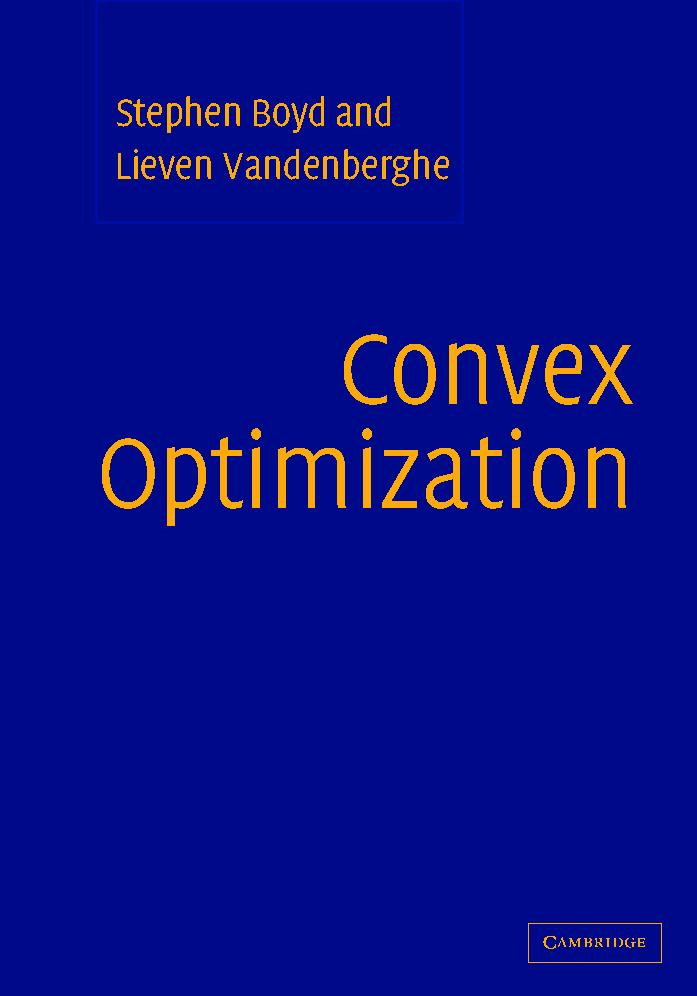
\includegraphics[height=0.6\textheight]{figures/bv_cvxbook_cover}
\par\end{center}

\end{frame}


\begin{frame}{What we will quickly review today}
  \tableofcontents
\end{frame}


\section{Convex Sets and Functions}

\begin{frame}{Notation from Boyd and Vandenberghe}
\begin{itemize}
\item $f:\reals^{p}\to\reals^{q}$ to mean that $f$ maps from some \emph{subset}
of $\reals^{p}$
\begin{itemize}
\item namely $\dom f\subset\reals^{p}$, where $\dom f$ is the domain of
$f$
\end{itemize}
\end{itemize}
\end{frame}



\mode<article>{What is the set $\left\{ \theta x_{1}+(1-\theta)x_{2}\mid\theta\in\reals\right\} $?
A line through $x_{1}$ and $x_{2}$. What is $\left\{ \theta x_{1}+(1-\theta)x_{2}\mid\theta\in[0,1]\right\} $?
The line segment conneting $x_{1}$ and $x_{2}$. }
\begin{frame}{Convex Sets}
\begin{definition}
A set $C$ is \textbf{convex} if for any $x_{1},x_{2}\in C$ and any
$\theta$ with $0\le\theta\le1$ we have
\[
\theta x_{1}+(1-\theta)x_{2}\in C.
\]
\end{definition}

\begin{center}
\includegraphics[height=0.45\textheight]{figures/{fig7.4a}.pdf}\includegraphics[height=0.45\textheight]{figures/{fig7.4b}.pdf}\let\thefootnote\relax\footnotetext{\tiny{KPM Fig. 7.4}}
\par\end{center}

\end{frame}

\begin{frame}{Convex and Concave Functions}
\begin{definition}
A function $f:\reals^{n}\to\reals$ is \textbf{convex} if $\dom f$
is a convex set and if for all $x,y\in\dom f$, and $0\le\theta\le1$,
we have
\[
f(\theta x+(1-\theta)y)\le\theta f(x)+(1-\theta)f(y).
\]
\end{definition}

\begin{center}
\includegraphics[height=0.45\textheight]{figures/{fig7.5a}.pdf}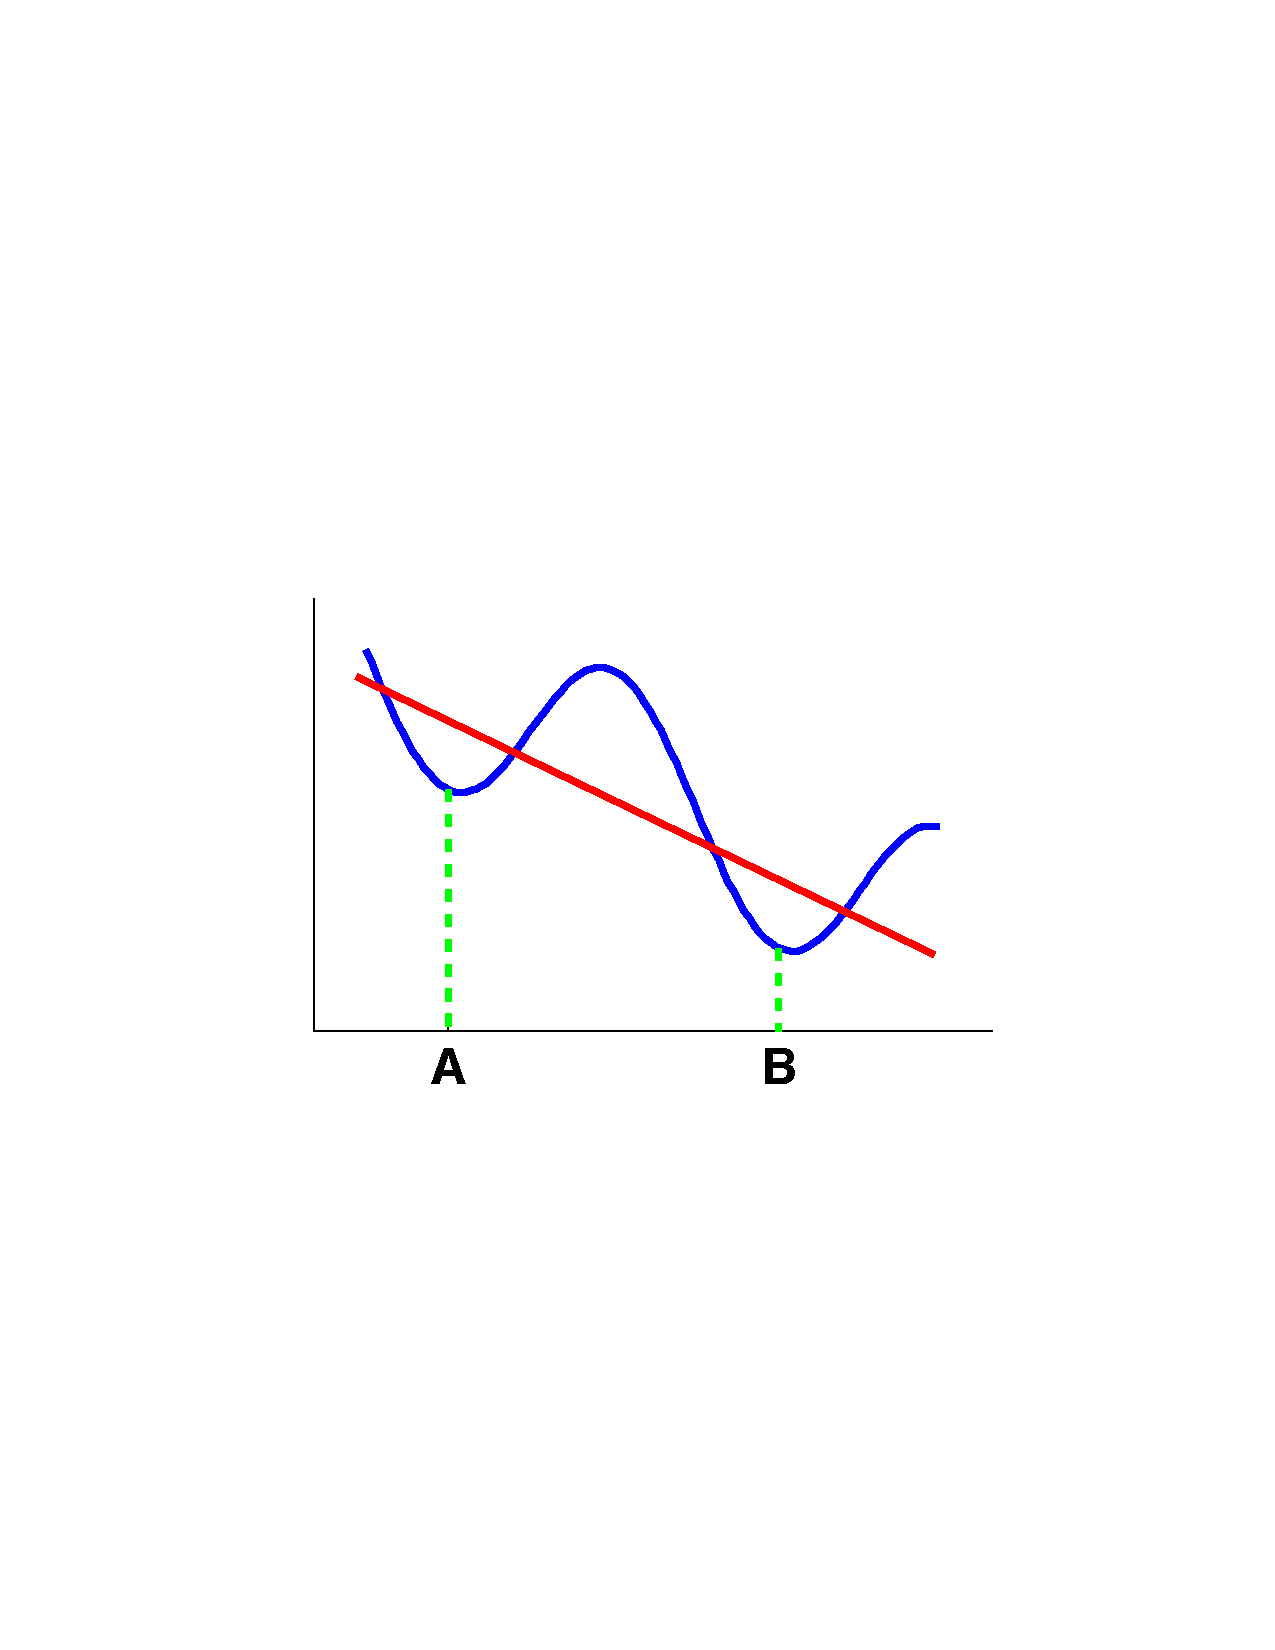
\includegraphics[height=0.45\textheight]{{figures/fig7.5b}.pdf}\let\thefootnote\relax\footnotetext{\tiny{KPM Fig. 7.5}}
\par\end{center}

\end{frame}

\begin{frame}{Examples of Convex Functions on $\reals$}
\begin{examples}

\begin{itemize}
\item $x\mapsto ax+b$ is both convex and concave on $\reals$ for all $a,b\in\reals$.

\pause{}
\item $x\mapsto\left|x\right|^{p}$ for $p\ge1$ is convex on $\reals$

\pause{}
\item $x\mapsto e^{ax}$ is convex on $\reals$ for all $a\in\reals$ 

\pause{}
\item Every norm on $\reals^{n}$ is convex (e.g. $\|x\|_{1}$ and $\|x\|_{2}$)

\pause{}
\item Max: $\left(x_{1},\ldots,x_{n}\right)\mapsto\max\left\{ x_{1}\ldots,x_{n}\right\} $
is convex on $\reals^{n}$
\end{itemize}
\end{examples}

\end{frame}

\begin{frame}{Convex Functions and Optimization}
\begin{definition}
A function $f$ is \textbf{strictly convex} if the line segment connecting
any two points on the graph of $f$ lies \textbf{strictly }above the
graph (excluding the endpoints).

\pause{}

\end{definition}

Consequences for optimization:
\begin{itemize}
\item \textbf{convex:} if there is a local minimum, then it is a \textbf{global}
minimum
\item \textbf{strictly convex:} if there is a local minimum, then it is
the \textbf{unique global} minumum
\end{itemize}
\end{frame}


\section{The General Optimization Problem}
\begin{frame}{General Optimization Problem: Standard Form}
\begin{block}{General Optimization Problem: Standard Form}
\begin{eqnarray*}
\textrm{minimize} &  & f_{0}(x)\\
\textrm{subject to} &  & f_{i}(x)\le0,\;\;i=1,\ldots,m\\
 &  & h_{i}(x)=0,\;\;i=1,\ldots p,
\end{eqnarray*}
where $x\in\reals^{n}$ are the \textbf{optimization variables }and\textbf{
}$f_{0}$ is the \textbf{objective function.}

\pause{}

\end{block}
Assume\textbf{ domain} $\cd=\bigcap_{i=0}^{m}\dom f_{i}\cap\bigcap_{i=1}^{p}\dom h_{i}$
is nonempty. 
\end{frame}

\begin{frame}{General Optimization Problem: More Terminology}
\begin{itemize}
\item The set of points satisfying the constraints is called the \textbf{feasible
set}.
\item A point $x$ in the feasible set is called a \textbf{feasible point.}

\pause{}

\item If $x$ is feasible and $f_{i}(x)=0$, 
\begin{itemize}
\item then we say the inequality constraint $f_{i}(x)\le0$ is \textbf{active}
at $x$.
\end{itemize}
\end{itemize}

\pause{}
\begin{itemize}
\item The \textbf{optimal value} $p^{*}$ of the problem is defined as
\[
p^{*}=\inf\left\{ f_{0}(x)\mid x\mbox{ satisfies all constraints}\right\} .
\]
\end{itemize}

\pause{}
\begin{itemize}
\item $x^{*}$ is an \textbf{optimal point} (or a solution to the problem)
if $x^{*}$ is feasible and $f(x^{*})=p^{*}$. 
\end{itemize}
\end{frame}

\begin{frame}{Do We Need Equality Constraints?}

\begin{itemize}
\item Consider an equality-constrained problem: 
\begin{eqnarray*}
\textrm{minimize} &  & f_{0}(x)\\
\textrm{subject to} &  & h(x)=0
\end{eqnarray*}
\end{itemize}

\pause{}
\begin{itemize}
  \item Note that
  \[
  h(x)=0\;\iff\;\left(h(x)\ge0\mbox{ AND}\;h(x)\le0\right)
  \]
\end{itemize}
  
\pause{}

\begin{itemize}
\item Can be rewritten as
\begin{eqnarray*}
\pause\textrm{minimize} &  & f_{0}(x)\\
\textrm{subject to} &  & h(x)\le0\\
 &  & -h(x)\le0.
\end{eqnarray*}
 
\end{itemize}

\pause{}
\begin{itemize}
\item For simplicity, we'll drop equality contraints from this presentation. 
\end{itemize}
\end{frame}


\section{Lagrangian Duality: Convexity not required}
\begin{frame}{The Lagrangian}

The general {[}inequality-constrained{]} optimization problem is:
\begin{eqnarray*}
\textrm{minimize} &  & f_{0}(x)\\
\textrm{subject to} &  & f_{i}(x)\le0,\;\;i=1,\ldots,m
\end{eqnarray*}

\begin{definition}

The \textbf{Lagrangian} for this optimization problem is
\[
L(x,\lambda)=f_{0}(x)+\sum_{i=1}^{m}\lambda_{i}f_{i}(x).
\]
\begin{itemize}
\item $\lambda_{i}$'s are called \textbf{Lagrange multipliers} (also called
the \textbf{dual variables}). 
\end{itemize}
\end{definition}

\end{frame}

\begin{frame}{The Lagrangian Encodes the Objective and Constraints}
\begin{itemize}
\item Supremum over Lagrangian gives back encoding of objective and constraints:
\begin{eqnarray*}
\sup_{\lambda\succeq0}L(x,\lambda) & = & \sup_{\lambda\succeq0}\left(f_{0}(x)+\sum_{i=1}^{m}\lambda_{i}f_{i}(x)\right)\\
\pause & = & \begin{cases}
f_{0}(x) & \mbox{when }f_{i}(x)\le0\;\mbox{all }i\\
\infty & \mbox{otherwise.}
\end{cases}
\end{eqnarray*}
\end{itemize}

\pause{}
\begin{itemize}
\item Equivalent \textbf{primal form} of optimization problem:
\[
p^{*}=\inf_{x}\sup_{\lambda\succeq0}L(x,\lambda)
\]
\end{itemize}
\end{frame}

\begin{frame}{The Primal and the Dual}
\begin{itemize}
\item Original optimization problem in  \textbf{primal form:}
\[
p^{*}=\inf_{x}\sup_{\lambda\succeq0}L(x,\lambda)
\]


\pause{}
\item Get the \textbf{Lagrangian dual problem} by ``swapping the inf and
the sup'':
\[
d^{*}=\sup_{\lambda\succeq0}\inf_{x}L(x,\lambda)
\]


\pause{}
\item We will show \textbf{weak duality}: $p^{*}\ge d^{*}$ for any optimization
problem
\end{itemize}
\end{frame}

\begin{frame}{Weak Max-Min Inequality}
\begin{theorem}
For \textbf{any} $f:W\times Z\to\reals$, we have
\[
\sup_{z\in Z}\inf_{w\in W}f(w,z)\le\inf_{w\in W}\sup_{z\in Z}f(w,z).
\]

\pause{}

\end{theorem}

% \begin{proof}
\textbf{Proof} \\
For any $w_{0}\in W$ and $z_{0}\in Z$, we clearly have
\[
\inf_{w\in W}f(w,z_{0})\le f(w_{0},z_{0})\le\sup_{z\in Z}f(w_{0},z).
\]

\pause{}

Since $\inf_{w\in W}f(w,z_{0})\le\sup_{z\in Z}f(w_{0},z)$ for all
$w_{0}$ and $z_{0}$, we must also have
\[
\sup_{z_{0}\in Z}\inf_{w\in W}f(w,z_{0})\le\inf_{w_{0}\in W}\sup_{z\in Z}f(w_{0},z).
\]
% \end{proof}

\end{frame}

\begin{frame}{Weak Duality}
\begin{itemize}
\item For any optimization problem (\textbf{not just convex}), weak max-min
inequality implies \textbf{weak duality}:
\end{itemize}
\begin{align*}
p^{*}= & \inf_{x}\sup_{\lambda\succeq0}\left[f_{0}(x)+\sum_{i=1}^{m}\lambda_{i}f_{i}(x)\right]\\
\ge & \sup_{\lambda\succeq0,\nu}\inf_{x}\left[f_{0}(x)+\sum_{i=1}^{m}\lambda_{i}f_{i}(x)\right]=d^{*}
\end{align*}


\pause{}
\begin{itemize}
\item The difference $p^{*}-d^{*}$ is called the \textbf{duality gap}.
\item For \emph{convex} problems, we often have \textbf{strong duality}:
$p^{*}=d^{*}$.
\end{itemize}
\end{frame}

\begin{frame}{The Lagrange Dual Function}
\begin{itemize}
\item The \textbf{Lagrangian dual problem}:
\[
d^{*}=\sup_{\lambda\succeq0}\inf_{x}L(x,\lambda)
\]


\pause{}

\end{itemize}
\begin{definition}
The \textbf{Lagrange dual function} (or just \textbf{dual function})
is 
\[
g(\lambda)=\inf_{x}L(x,\lambda)=\inf_{x}\left(f_{0}(x)+\sum_{i=1}^{m}\lambda_{i}f_{i}(x)\right).
\]

\pause{}
\end{definition}

\begin{itemize}
\item The dual function may take on the value $-\infty$ (e.g. $f_{0}(x)=x$).

\pause{}
\item The dual function is always \textbf{concave}
\begin{itemize}
\item since pointwise min of affine functions
\end{itemize}
\end{itemize}
\end{frame}

\begin{frame}{The Lagrange Dual Problem: Search for Best Lower Bound}
\begin{itemize}
\item In terms of Lagrange dual function, we can write weak duality as
\begin{align*}
p^{*} & \ge\sup_{\lambda\ge0}g(\lambda)=d^{*}
\end{align*}


\pause{}
\item So for any $\lambda$ with $\lambda\ge0$, \textbf{Lagrange dual function
gives a lower bound on optimal solution}:
\[
p^{*}\ge g(\lambda)\text{ for all }\lambda\ge0
\]
 
\end{itemize}
\end{frame}

\begin{frame}{The Lagrange Dual Problem: Search for Best Lower Bound}
 
\begin{itemize}
\item The \textbf{Lagrange dual problem} is a search for best lower bound
on $p^{*}$:
\begin{eqnarray*}
\textrm{maximize} &  & g(\lambda)\\
\textrm{subject to} &  & \lambda\succeq0.
\end{eqnarray*}


\pause{}
\begin{itemize}
\item $\lambda$ \textbf{dual feasible} if $\lambda\succeq0$ and $g(\lambda)>-\infty$.

\pause{}
\item $\lambda^{*}$ \textbf{dual optimal} or \textbf{optimal Lagrange multipliers}
if they are optimal for the Lagrange dual problem. 

\pause{}
\end{itemize}
\item Lagrange dual problem often easier to solve (simpler constraints).

\pause{}
\item $d^{*}$ can be used as stopping criterion for primal optimization.

\pause{}
\item Dual can reveal hidden structure in the solution.
\end{itemize}
\end{frame}

\begin{frame}{Recap Lagrangian Duality}
  \begin{itemize}
    \item {\bf Lagrangian} $L(x,\lambda)=f_{0}(x)+\sum_{i=1}^{m}\lambda_{i}f_{i}(x),$ with $\lambda_i$ multipliers / dual variables
    \pause{}
    \item Equivalence to original optimization problem:
    \begin{align*}
      \begin{aligned}
        \textrm{minimize} & \quad  f_{0}(x)\\
      \textrm{subject to} & \quad  f_{i}(x)\le0,\;\;i=1,\ldots,m
      \end{aligned} \qquad \Rightarrow  p^{*} = \inf_{x}\sup_{\lambda\succeq0}\left[L(x, \lambda)\right] 
    \end{align*}
    \pause{}
    \item {\bf Weak duality} $ p^{*} \ge \sup_{\lambda\succeq0,\nu}\inf_{x}\left[L(x, \lambda)\right]=d^{*} $
    \pause{}
    \item {\bf Dual function}  $g(\lambda)=\inf_{x}L(x,\lambda)=\inf_{x}\left(f_{0}(x)+\sum_{i=1}^{m}\lambda_{i}f_{i}(x)\right)$ is always concave
    \pause{}
    \item Convex problems ($f_i$ convex) have {\bf strong duality} $p^{*} = d^{*}$
  \end{itemize}
\end{frame}


\section{Convex Optimization}

\begin{frame}{Convex Optimization Problem: Standard Form}
\begin{block}{Convex Optimization Problem: Standard Form}
\begin{eqnarray*}
\textrm{minimize} &  & f_{0}(x)\\
\textrm{subject to} &  & f_{i}(x)\le0,\;\;i=1,\ldots,m
\end{eqnarray*}
where $f_{0},\ldots,f_{m}$ are convex functions. 

\end{block}
\end{frame}

\begin{frame}{Strong Duality for Convex Problems}
\begin{itemize}
\item For a convex optimization problems, we \textbf{usually} have strong
duality, but not always. 
\begin{itemize}
\item \let\thefootnote\relax\footnotetext{\tiny{Example from Laurent El Ghaoui's EE 227A: Lecture 8 Notes, Feb 9, 2012}}For
example:
\begin{eqnarray*}
\textrm{minimize} &  & e^{-x}\\
\textrm{subject to} &  & x^{2}/y\le0\\
 &  & y>0
\end{eqnarray*}
 
\end{itemize}
\item The additional conditions needed are called \textbf{constraint qualifications}. 
\end{itemize}
\end{frame}

\begin{frame}{Slater's Constraint Qualifications for Strong Duality}
\begin{itemize}
\item Sufficient conditions for strong duality in a \textbf{convex} problem. 

\pause{}
\item Roughly: the problem must be \textbf{strictly }feasible.

\pause{}
\item Qualifications when problem domain\footnote{$\cd$ is the set where all functions are defined, NOT the feasible
set.} $\cd\subset\reals^{n}$ is an open set:

\begin{itemize}
\item \textbf{Strict feasibility is sufficient}. ($\exists x$ $f_{i}(x)<0$
for $i=1,\ldots,m$)
\item For any affine inequality constraints, $f_{i}(x)\le0$ is sufficient. 

\pause{}
\end{itemize}
\item Otherwise, see notes or BV Section 5.2.3, p. 226. 
\end{itemize}
\end{frame}


\section{Complementary Slackness}
\begin{frame}{Complementary Slackness}
\begin{itemize}
\item Consider a general optimization problem (i.e. not necessarily convex).

\pause{}
\item If we have \textbf{strong duality}, we get an interesting relationship
between
\begin{itemize}
\item the optimal Lagrange multiplier $\lambda_{i}$ and
\item the $i$th constraint at the optimum: $f_{i}(x^{*})$

\pause{}
\end{itemize}
\item Relationship is called ``\textbf{complementary slackness}'':
\[
\lambda_{i}^{*}f_{i}(x^{*})=0
\]


\pause{}
\item Always have Lagrange multiplier is zero \textbf{or} constraint is
active at optimum \textbf{or} both.
\end{itemize}
\end{frame}

\begin{frame}{Complementary Slackness ``Sandwich Proof''}
\begin{itemize}
\item Assume strong duality: $p^{*}=d^{*}$ in a general optimization problem
\item Let $x^{*}$ be primal optimal and $\lambda^{*}$ be dual optimal.
Then:
\begin{eqnarray*}
f_{0}(x^{*}) & = & g(\lambda^{*})=\inf_{x}\,L(x,\lambda^{*})\pause\text{\quad(strong duality and definition)}\\
\pause & \le & L(x^{*},\lambda^{*})\\
\pause & = & f_{0}(x^{*})+\sum_{i=1}^{m}\underbrace{\lambda_{i}^{*}f_{i}(x^{*})}_{\le0}\\
\pause & \le & f_{0}(x^{*}).
\end{eqnarray*}


\pause{}

\end{itemize}
Each term in sum $\sum_{i=1}\lambda_{i}^{*}f_{i}(x^{*})$ must actually
be $0$. That is
\[
\boxed{\lambda_{i}^{*}f_{i}(x^{*})=0,\quad i=1,\ldots,m}.
\]
This condition is known as \textbf{complementary slackness}. 
\end{frame}
%
\begin{frame}{Result of ``Sandwich Proof'' and Consequences}
\begin{itemize}
\item Let $x^{*}$ be primal optimal and $\lambda^{*}$ be dual optimal. 
\item If we have strong duality, then 
\[
p^{*}=d^{*}=f_{0}(x^{*})=g(\lambda^{*})=L(x^{*},\lambda^{*})
\]
and we have {\bf complementary slackness}
\end{itemize}
\[
\lambda_{i}^{*}f_{i}(x^{*})=0,\quad i=1,\ldots,m.
\]


\pause{}
\begin{itemize}
\item From the proof, we can also conclude that
\[
L(x^{*},\lambda^{*})=\inf_{x}L(x,\lambda^{*}).
\]
\end{itemize}

\pause{}
\begin{itemize}
\item If $x\mapsto L(x,\lambda^{*})$ is differentiable, then we must have
$\del L(x^{*},\lambda^{*})=0$.
\end{itemize}
\end{frame}

\end{document}